\documentclass[a4paper,12pt]{mwart}

\usepackage{polski}
\usepackage[utf8]{inputenc}
\usepackage{float}
\usepackage{color}
\usepackage{hyperref}
\usepackage{tikz}
\usetikzlibrary{arrows,positioning,automata}
\tikzset{>=stealth',shorten >=1pt,auto,thick,main node/.style={rectangle,fill=blue!30,draw,minimum size=0.8cm,inner sep=10pt,font=\sffamily\large\bfseries},edge/.style={thick,double}}
\usepackage{enumitem}

\newcommand{\TODO}[1]{\textcolor{blue}{TODO: #1 \\}}
\newcommand{\ang}[1]{ang.~{\itshape #1}}

% http://tex.stackexchange.com/questions/83440/inputenc-error-unicode-char-u8-not-set-up-for-use-with-latex
\DeclareUnicodeCharacter{00A0}{~}

\begin{document}

\title{Cebula Deal Finder\\%
{\large czyli system wykrywania okazji sprzedażowych w Internecie} }

\author{Łukasz ,,Cebula'' Jędrzejewski \and Igor ,,Prohibicja'' Rodzik \and Artur ,,Pieseł'' Sawicki}

\maketitle

\section{Opis projektu}
W ramach projektu realizujemy system służący do wykrywania okazji sprzedażowych w internecie. Produktami, jakich ceny porównujemy, są książki.
Program znajduje wpisany przez użytkownika tytuł na paru serwisach internetowych (zaimplementowanych mamy cztery:
\href{http://www.empik.com}{empik.com}, \href{http://www.ksiegarniawarszawa.pl}{ksiegarniawarszawa.pl}, \href{http://www.matras.pl}{matras.pl} i \href{http://www.aros.pl}{aros.pl}
), dopasowuje znalezione pozycje, a następnie porównuje ich ceny i prezentuje je użytkownikowi.

\section{Architektura}
Do realizacji projektu użyliśmy języka scala oraz frameworka Akka do tworzenia i zarządzania aktorami.
Poniższe sekcje opisują stworzonych przez nas aktorów oraz interakcje między nimi.

\begin{figure}[H]
  \centering
  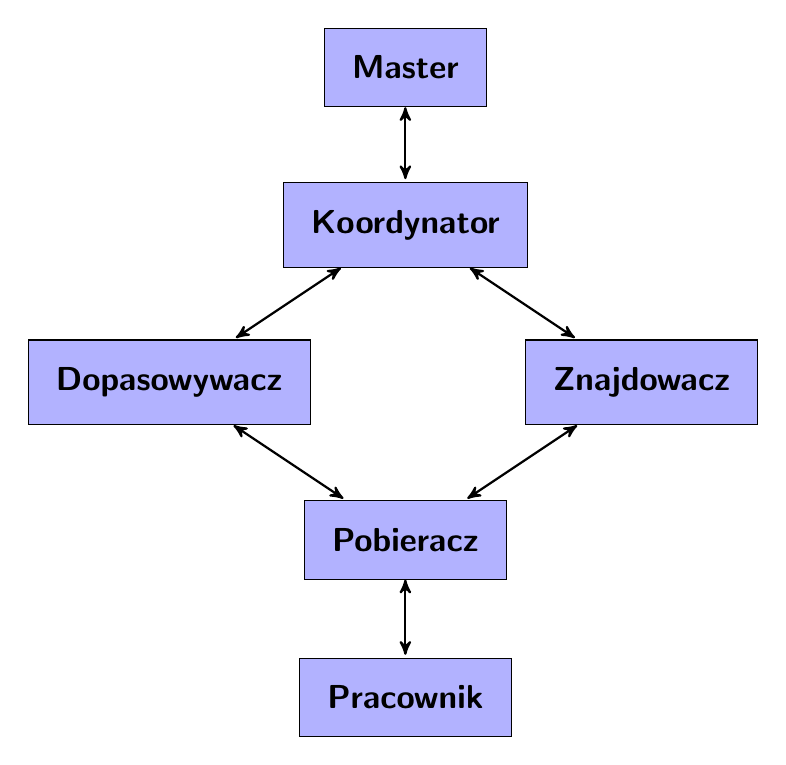
\begin{tikzpicture}
    \node[main node, on grid] (v1) {Master};
    \node[main node, on grid] (v2) [below = 2cm of v1]  {Koordynator};
    \node[main node, on grid] (v3) [below right = 2cm and 3cm of v2] {Znajdowacz};
    \node[main node, on grid] (v4) [below = 6cm of v1] {Pobieracz};
    \node[main node, on grid] (v5) [below left = 2cm and 3cm of v2] {Dopasowywacz};
    \node[main node, on grid] (v6) [below = 2cm of v4] {Pracownik};
    \path[edge] (v1) edge [<->] node {} (v2);
    \path[edge] (v2) edge [<->] node {} (v3);
    \path[edge] (v2) edge [<->] node {} (v5);
    \path[edge] (v3) edge [<->] node {} (v4);
    \path[edge] (v5) edge [<->] node {} (v4);
    \path[edge] (v4) edge [<->] node {} (v6);
  \end{tikzpicture}
  \caption{Dragram prezentujący interakcje między aktorami}
\end{figure}

\subsection{Władca (\ang{Master})}
Od tego aktora rozpoczyna się interakcja użytkownika z aplikacją. Jego zadaniem jest przyjęcie tytułu do wyszukiwania i przekazanie pracy nowemu koordynatorowi,
a także odbiór wyników pracy od koordynatora i ich prezentacja.

Nowy koordynator tworzony jest per tytuł do wyszukania.

\subsection{Koordynator (\ang{Coordinator})}
Koordynator tworzony jest per wyszukiwany przez użytkownika tytuł. Do jego obowiązków należy przekazanie tytułu do wyszukiwania poszczególnym znajdowaczom,
zebranie wyników od wszystkich znajdowaczy, przekazanie ofert do dopasowania do dopasowywacza i, finalnie, zwrócenie pogrupowanych pozycji do mastera.

\subsection{Znajdowacz (\ang{Finder})}
Każdy z serwisów, na których wyszukujemy książki, ma zaimplementowanego znajdowacza właściwego sobie. Każdy z nich potrafi zebrać ze strony listę wyników wyszukiwania,
a następnie z każdej podstrony zbudować jednolity rezultat oferty. Listę ofert oddaje koordynatorowi. Do pobierania stron każdy ze znajdowaczy korzysta z pobieracza.

\subsection{Pobieracz (\ang{Downloader})}
Zadanie pobieracza to rozdzielanie żądań pobierania między dostępnych pracowników (\ang{worker}), z których każdy pobiera stronę o podanym adresie URL.
Pobieracz jest tylko jeden na całą aplikację i kontroluje on pulę pracowników pobierających konkretne strony. Pozwala to ograniczyć liczbę utrzymywanych połączeń HTTP.
Liczbę pracowników ustawiliśmy na 5, jednak można ją zmienić w zależności od potrzeb użytkownika.

\subsection{Dopasowywacz (\ang{Matcher})}
Dopasowywacz potrafi pogrupować otrzymane ze wszystkich serwisów oferty, tak aby móc je porównać i zaprezentować użytkownikowi.
Korzysta w tym celu z algorytmu {\itshape k-medoid}, który zostanie opisany poniżej.

\section{Dopasowywanie ofert}
Dopasowywanie ofert wymagało od nas użycia metod z zakresu przetwarzania tekstu oraz eksploracji danych tekstowych.

\subsection{Przygotowanie danych}
Pierwszym krokiem dopasowania było przygotowanie danych. Na początku z opisu
zostały przekształcone na wektory słów. Wszystkie znaki białe oraz znaki
przestankowe zostały zignorowane. Następnie zastosowana została lista słów stopu,
która zawierała słowa nieistotne takie jak łączniki zdań. Bazą dla naszej listy
była lista słów stopu Wikipedii. Tak przefiltrowany wektor mógł być przekazany
do następnego etapu.

\subsection{Algorytm k-medoid}

Zaimplementowanym algorytmem do~grupowania danych jest \emph{k-medoid}. Jest
on~podobny do~algorytmu k-średnich, jednak punkty wyznaczające grupy
(\emph{medoidy}) są~przykładami ze~zbioru danych. Pozwala to~na~uniknięcie
konieczności określenia sposobu w~jaki można stworzyć pośrednie punkty
wyznaczające centra (w~naszym przypadku wektory wyrazów).

Algorytm działa następująco:

\begin{enumerate}
\item Wylosuj $k$ przykładów, które będą medoidami. $k$ to~pożądana liczba
  grup.
\item Dopóki suma odległości do~medoid maleje i~nie osiągnięto liczby
  zadanych iteracji:
\begin{enumerate}[label*=\arabic*.]
\item Dla każdego medoida i~dla każdego przykładu:
\begin{enumerate}[label*=\arabic*.]
\item Zamień bieżącego medoida na~aktualny przykład.
\item Oblicz sumę odległości do~medoid.
\item Jeśli się zwiększyła, wycofaj zamianę.
\end{enumerate}
\end{enumerate}
\end{enumerate}

Algorytm do~porównywania podobieństwa przykładów wykorzystuje miarę odległości.
Dwie z~nich opisaliśmy w~kolejnej sekcji.

Podczas badania zachowania algorytmu zauważyliśmy, że~oblicza on~miary
odległości dla par przykładów wielokrotnie. Wobec tego dodaliśmy zapamiętywanie
wyników miary odległości dla każdego wywołania. Przyspieszyło to~proces
grupowania aż~kilkanaście razy.

\subsection{Miara odległości}

Zaimplementowane miary porównują niepodobieństwo dwóch wektorów wyrazów.
Im~wartość bliższa 0, tym bardziej dwa wektory są~podobne.

\subsubsection{N-gramy}
N-gramy to n-elementowe ciągi kolejnych słów z rozpatrywanego wektora. Dzięki
analizie ciągów a nie tylko pojedynczych słów, pod uwagę brana jest również
zależność między wyrazami. Następnie porównuje się występowanie poszczególnych
n-gramów w przetwarzanych dokumentach. Dokumenty, które mają najwięcej wspólnych
n-gramów należą do tej samej grupy.

\subsubsection{Miara kosinusowa i~TFIDF}

Kolejną miarą jest miara kosinusowa połączona z~miarą TFIDF.

Miara TFIDF ma~na~celu wyznaczenie wag wyrazów w~dokumencie. W~taki sposób, aby
uwzględnić występowanie wyrazu w~dokumencie (miara tf), jaki i~wszystkich
dokumentach (idf). W~ten sposób wyrazy pospolite we~wszystkich dokumentach będą
miały niską wagę. Z~kolei te~obecne w~niewielkiej części, wyższą.

Takie wektory porównujemy miarą kosinusową.

Ostatecznie używamy tej miary, gdyż okazała się być nieco trafniejsza.

\subsection{Wybór liczby grup}

W~zagadnieniu grupowania duży problem stanowi odpowiedni wybór liczby grup.
Czasem zdarza się, że~wiemy z~góry ile ich powinno być. Jednak w~naszym
projekcie stanęliśmy przed koniecznością wyboru liczby grup automatycznie.

Pierwszym rozwiązaniem, które opracowaliśmy było uruchomienie algorytmu
grupowania danych dla zakresu grup $[2, \lceil \frac{n}{2} \rceil]$, gdzie $n$
to~liczba przykładów. Po~wyznaczeniu grup, sprawdzaliśmy sumy średnich
odległości między przykładami w~klastrach. Im~opisana suma była mniejsza, tym
grupowanie traktowaliśmy za~lepsze. Mankamentem tego sposobu oceny jest fakt,
że~każde grupowanie dla większej liczby grup, będzie lepsze. W~szczególności
dla grupowania, w~którym liczba przykładów pokrywa się z~liczbą grup, miara
oceny wyniesie $0$.

W~związku z~tym postanowiliśmy skorzystać z~jednej dostępnych metod oceny
jakości grupowania, która nie wymaga wiedzy o~\textbf{prawdziwych}
przypisaniach do~grup. Zaimplementowaliśmy miarę sylwetki (\ang{silhouette}).
Jej idea polega na~skonfrontowaniu średniej niepodobieństw do~przykładów
z~takiego samego klastra, jak rozważany przykład -- $a(i)$, gdzie $i$
to~przykład, oraz najmniejszej średniej niepodobieństw przykładów należących
do~pozostałych klastrów -- $b(i)$. Następnie zdefiniowany jest wskaźnik:

\[s(i) = \frac{b(i) - a(i)}{\max[a(i), b(i)]}\]

którego najbardziej pożądana wartość powinna być bliska $1$, co~oznacza,
że~przykład jest znacznie bliższy przykładom w~grupie, do~której należy, niż
do~jakiejkolwiek z~innych grup. Taka sytuacja zachodzi dla $a(i) \ll~b(i)$.

Wartość miary sylwetki należy do~przedziału $[-1, 1]$, co~kłóciło się
z~przyjętym w~projekcie założeniem, że~im~mniejsza wartość tym lepsze
grupowania. Dlatego zmodyfikowaliśmy miarę następująco:

\[s'(i) = \left | s(i) - 1 \right | \]

Ostatecznie zależało nam na~wskaźniku dla całego grupowania, dlatego powyższą
wartość uśredniamy na~wszystkich przykładach.

Po~zastosowaniu miary sylwetki do~wyboru najlepszego efekty nie były dużo
lepsze od~pierwszego sposobu oceny. Co~prawda dla niewielkiej liczby grup,
wartość miary była dość zróżnicowana, to~jednak wraz ze~wzrostem liczby
klastrów, ciągle malała.

Ta~obserwacja skłoniła nas do~dodania wpływu wielkości grupy na~miarę.
Zmieniliśmy tylko formułę $a(i)$, czyli średnią odległość przykładu do~innych
przykładów w~jego grupie, w~poniższy sposób:

\begin{itemize}
\item grupy jednoelementowe karzemy -- zwracamy $0{,}1$, zamiast $0$
  w~oryginalnej mierze,
\item z~kolei większe grupy zdecydowaliśmy się promować -- zwracamy $a(i) /
  \left (1 + \log_{10} \left | C(i) \right | \right)$, gdzie $\left | C(i)
  \right |$ to~liczba przykładów w~grupie przykładu $i$, dzieląc przez czynnik
  zależny od~liczności grupy.
\end{itemize}

Dopiero tak zmodyfikowana miara sylwetki przyniosła pewną poprawę.

\section{Demonstracja działania}

Poniższy wycinek logów pokazuje działanie programu i~końcowy rezultat dla
zapytania ,,pustynna włócznia''.

\scriptsize
\begin{verbatim}
[info] Running cdf.main.Main pustynna włócznia
[.../master/coordinator1/empikFinder] Received pustynna włócznia query to search in Empik
[.../master/coordinator1/matrasFinder] Received pustynna włócznia query to search in Matras
[.../master/coordinator1/arosFinder] Received pustynna włócznia query to search in Aros
[.../master/coordinator1/kwFinder] Received pustynna włócznia query to search in Księgarnia Warszawa
[.../master/downloader] Received url http://aros.pl/szukaj/pustynna+włócznia/0 to download. Routing
[.../master/downloader/downloadWorker3] Received url http://aros.pl/szukaj/pustynna+włócznia/0 to download
[.../master/coordinator1/arosFinder] Found List(http://aros.pl/ksiazka/pustynna-wlocznia-ksiega-1-3, ...)
[.../master/downloader] Received url http://aros.pl/ksiazka/pustynna-wlocznia-ksiega-1-3 to download. Routing
[.../master/downloader/downloadWorker4] Received url https://ksiegarniawarszawa.pl/produkt/11894 to download
[.../master/coordinator1] Received offers
 Vector(Offer(http://aros.pl/ksiazka/pustynna-wlocznia-ksiega-1-3, Pustynna włócznia. Księga 1, ...), ...)
[.../master/coordinator1] All received offers are
...
(5,Offer(http://aros.pl/ksiazka/pustynna-wlocznia-ksiega-1-3, Pustynna włócznia. Księga 1, Peter V. Brett, 29.13))
...
For k = 11 clustering is Vector(8, 8, ...) with overall distance = 10.072649533170214
 and validation = 0.25774049370767016 for offers ...
[.../master] Offers groups
group 0
  0 Offer(https://ksiegarniawarszawa.pl/produkt/8272, Włócznia przeznaczenia, Arnaud Delalande, 8.19)
group 1
  0 Offer(http://aros.pl/ksiazka/pustynna-burza-scooby-doo-na-tropie-komiksow-14, ...)
group 2
  0 Offer(https://ksiegarniawarszawa.pl/produkt/11894, Pustynna gorączka, Diana Palmer, 8.12)
group 3
  0 Offer(https://ksiegarniawarszawa.pl/produkt/236520, Włócznia, Louis De Wohl, 39.9)
group 4
  0 Offer(http://aros.pl/ksiazka/maly-konstruktor---pustynna-burza-goliath-alex, ...)
  1 Offer(http://aros.pl/ksiazka/maly-konstruktor---pustynna-burza-hunter-alex, ...)
  2 Offer(http://aros.pl/ksiazka/maly-konstruktor---pustynna-burza-cobra-alex, ...)
group 5
  0 Offer(http://aros.pl/ksiazka/pustynna-wojna-rommla, Pustynna wojna Rommla, Kitchen Martin, 34.3)
  1 Offer(https://ksiegarniawarszawa.pl/produkt/248713, Pustynna wojna Rommla. II wojna światowa w ...)
  2 Offer(http://www.matras.pl/pustynna-wojna-rommla-ii-wojna-swiatowa-w-afryce-polnocnej-1941-1943,p,203086 ...)
group 6
  0 Offer(https://ksiegarniawarszawa.pl/produkt/112460, Pustynna odyseja, Harvey Lilley, 8.19)
group 7
  0 Offer(https://ksiegarniawarszawa.pl/produkt/16591, Pustynna Włócznia. Księga 2, Peter V. Brett, 32.72)
  1 Offer(https://ksiegarniawarszawa.pl/produkt/10178, Pustynna włócznia. Księga 2, Peter U.brett, 36.16)
group 8
  0 Offer(https://ksiegarniawarszawa.pl/produkt/7078, Włócznia przeznaczenia, Craig Smith, 28.62)
group 9
  0 Offer(https://ksiegarniawarszawa.pl/produkt/17322, Pustynna włócznia. Księga 1, Peter U.brett, 28.62)
  1 Offer(http://aros.pl/ksiazka/pustynna-wlocznia-ksiega-1-3, Pustynna włócznia. Księga 1, Peter V. Brett, 29.13)
  2 Offer(https://ksiegarniawarszawa.pl/produkt/121000, Pustynna włócznia. Księga 1, Peter V. Brett, 32.72)
  3 Offer(http://www.matras.pl/pustynna-wlocznia-ksiega-1,p,228819,
          Pustynna włócznia. Księga 1, Peter V. Brett, 33.38)
  4 Offer(http://www.empik.com/pustynna-wlocznia-ksiega-1-brett-peter-v,prod57795561,ksiazka-p,
          Pustynna włócznia. Księga 1, Brett Peter V., 35.99)
group 10
  0 Offer(http://www.matras.pl/pustynna-burza-pierwsza-wojna-nad-zatoka-perska-1991,p,223873, ...)
\end{verbatim}
\normalsize

Jak widać, pogrupowanie wyników wyszukiwania dla tego przykładu jest w~zasadzie
bezbłędne.

\section{Podsumowanie}
Systemy agentowe to bardzo ciekawe podejście do projektowania i implementacji
aplikacji rozproszonych. Pozwala ono na łatwe i skuteczne zarządzanie aplikacją
rozlokowaną na różnych maszynach. Framework Akka doskonale spisuje się w roli
frameworka do zastosowań agentowych, umożliwia zastosowanie bardziej
zaawansowanych technik interakcji z agentami, takich jak zastosowany przez nas
routing.

Mamy jednak kilka zastrzeżeń do języka Scala. Język ten sam w sobie
jest doskonałym narzędziem do pracy, jednak część jego mechanizmów zamiast
założonego przez twórców uproszczenia kodu, zdaje się jedynie go zaciemniać
(przede wszystkim słowo kluczowe \verb+implicit+).
Irytujący jest również czas kompilacji oraz o wiele gorsze wsparcie IDE niż
w przypadku języka Java.

Jeśli chodzi o część związaną z eksploracją tekstu, jedyny problem stanowiło
dopasowywanie ofert, jednak po kilku próbach udało nam się znaleźć
satsfakcjonujące rozwiązanie.

Podsumowując, stworzyliśmy działającą, rozproszoną aplikację
realizującą cel projektu. Dzięki temu nabyliśmy wiedzę, którą możemy wykorzystać
nie tylko w projektach uczelnianych, ale również w pracy.

\end{document}
